% Original prompt-and-response captures, explained in Section 2.
\section{AI Interaction Evidence}
\label{sec:d}

The first interaction concerns the beach-line and event-queue invariants. Its response explains why rotations preserve arc order and why generation counters invalidate obsolete circle predictions. The guard is checked by the retained stale-event regressions.

\begin{figure}[!htbp]
\centering
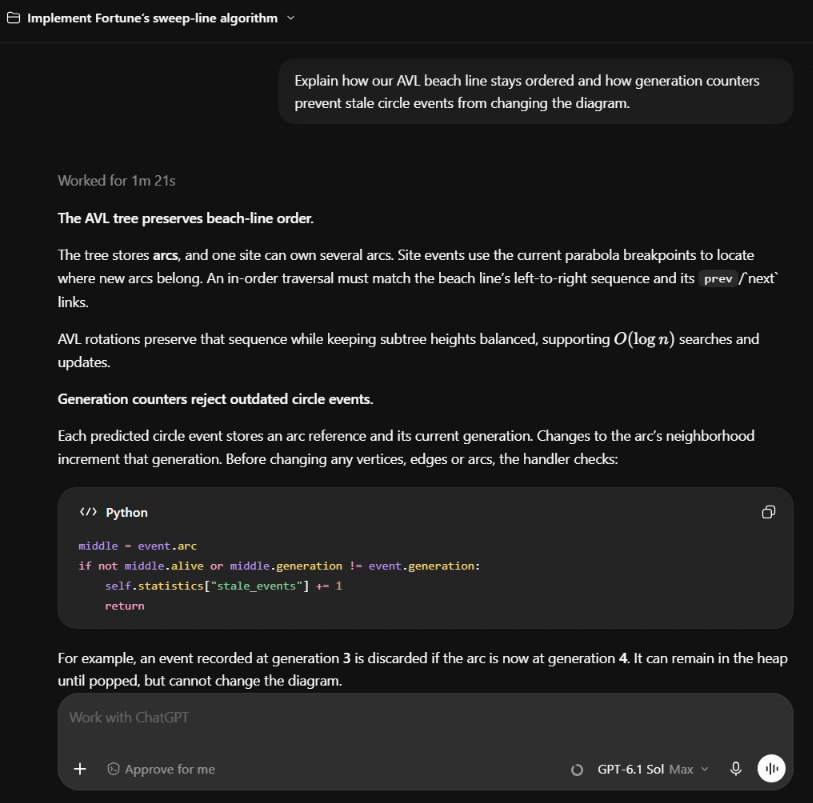
\includegraphics[width=0.99\linewidth,height=0.73\textheight,keepaspectratio]{ai-interaction-1.png}
\caption{ChatGPT prompt and response explaining AVL order and stale circle-event rejection.}
\label{fig:ai-chatgpt}
\end{figure}

\clearpage
\begin{landscape}
\thispagestyle{empty}
\captionsetup{hypcap=false}
\centering
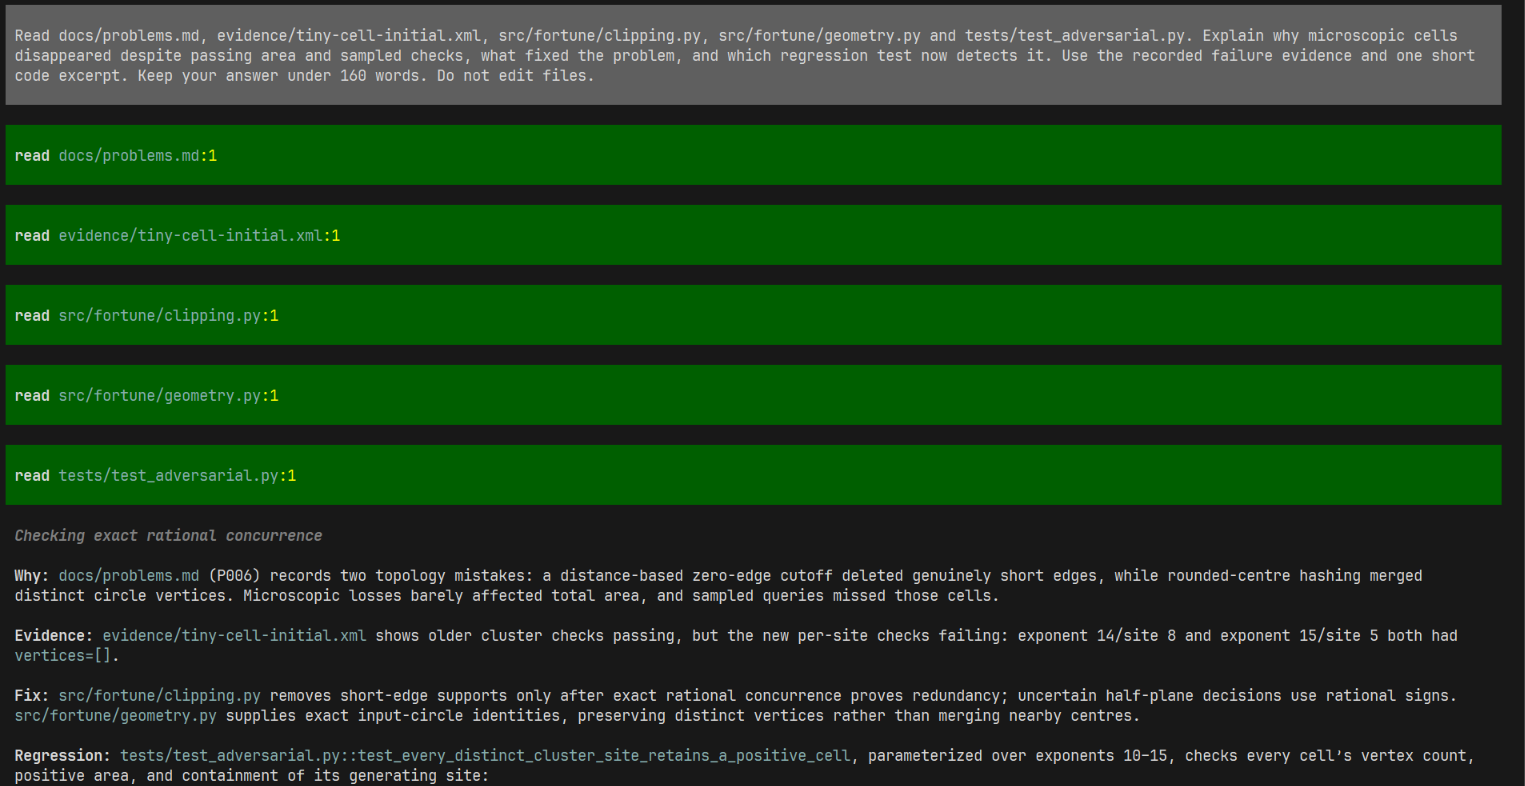
\includegraphics[width=\linewidth,height=116mm,keepaspectratio]{ai-interaction-2.png}\par
\vspace{2mm}
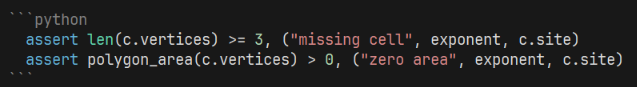
\includegraphics[width=115mm,height=16mm,keepaspectratio]{pi-tiny-cell-code-continuation.png}\par
\captionof{figure}{Pi prompt and response investigating microscopic cells, followed by the per-site regression excerpt.}
\label{fig:ai-pi}
\vspace{2mm}
{\fontsize{10}{12}\selectfont\thepage\par}
\end{landscape}
